\documentclass[aspectratio=169,10pt]{beamer}
\usepackage[T1]{fontenc}
\usepackage[utf8]{inputenc}
% babel indisponível neste ambiente; no seu LaTeX use \usepackage[brazil]{babel}
\renewcommand{\proofname}{Prova}
\usepackage{amsmath,amssymb,amsthm}
\usepackage{tikz}
\usetikzlibrary{shapes.geometric,arrows.meta}
\usetikzlibrary{positioning,decorations.pathreplacing}
\usepackage{algpseudocode}
\algtext*{EndFor}
\algtext*{EndWhile}
\algtext*{EndIf}

\usetheme{Madrid}
\setbeamertemplate{navigation symbols}{}
\setbeamertemplate{footline}[frame number]
\setbeamertemplate{enumerate items}[default]
\setbeamerfont{block title}{size=\small}

% ---------- macros ----------
\newcommand{\Cria}{\mathtt{cria}}
\newcommand{\Busca}{\mathtt{busca}}
\newcommand{\Uniao}{\mathtt{uniao}}
\newcommand{\Link}{\mathtt{link}}
\renewcommand{\lg}{\operatorname{lg}}
\newcommand{\lgs}{\lg^{*}}
\tikzset{>=Stealth}

% ---------- pseudocódigo em português ----------
\algrenewcommand\algorithmicrequire{\textbf{Entrada:}}
\algrenewcommand\algorithmicwhile{\textbf{enquanto}}
\algrenewcommand\algorithmicdo{\textbf{faça}}
\algrenewcommand\algorithmicfor{\textbf{para}}
\algrenewcommand\algorithmicforall{\textbf{para cada}}
\algrenewcommand\algorithmicif{\textbf{se}}
\algrenewcommand\algorithmicthen{\textbf{então}}
\algrenewcommand\algorithmicelse{\textbf{senão}}
\algrenewcommand\algorithmicend{\textbf{fim}}
\algrenewcommand\algorithmicreturn{\textbf{devolva}}
\algrenewcommand\alglinenumber[1]{\scriptsize #1:}
\algrenewcommand\algorithmiccomment[1]{\hfill$\triangleright$ #1}

\title[Conjuntos disjuntos]{Estruturas de dados para conjuntos disjuntos}
\subtitle{União-e-busca (\textit{union-find}) e a análise do algoritmo de Kruskal}
\author{Jair}
\institute{CMCC -- UFABC}
\date{}

\begin{document}

\begin{frame}[plain]
  \titlepage
\end{frame}

% % =====================================================================
% \begin{frame}{Roteiro}
%   \begin{enumerate}
%   \item Onde aparecem os conjuntos disjuntos: o algoritmo de Kruskal
%   \item O problema e as três operações $\Cria$, $\Busca$, $\Uniao$
%   \item Representação por \textbf{vetor}: simples, mas $\Theta(n)$ por
%     união
%   \item Representação por \textbf{listas ligadas} e a heurística da menor lista
%   \item Representação por \textbf{floresta}: união por tamanho/altura
%   \item Floresta com \textbf{rank} e \textbf{compressão de caminhos}
%   \item Análise: $O((m+n)\lgs n)$ (e o teorema de Tarjan, $O(m\,\alpha(m,n))$)
%   \end{enumerate}
% \end{frame}
% 
 % =====================================================================
 \begin{frame}[c]{Kruskal: onde aparecem os conjuntos disjuntos}

   Enquanto $S$ evolui de $\emptyset$ até uma árvore geradora, $(V,S)$
   é sempre uma \textbf{subfloresta geradora} de $G$.  Para
   $e=\{x,y\}\notin S$:
   \[
     (V,S\cup\{e\})\ \text{é acíclico}\iff
     {   x\text{ e }y\text{ estão em subconjuntos disjuntos de }V.}
   \]

   \medskip

   {Logo, o teste de aciclicidade do Kruskal equivale a verificar se $e$
   não liga vértices do mesmo conjunto da partição; ao inserir $e$ em
   $S$, \textbf{unimos} o conjunto de $x$ com o de $y$.}
 
   \medskip

   $\Rightarrow$ precisamos de estruturas que representem e manipulem,
   dinamicamente, conjuntos disjuntos de modo eficiente:
   \textit{union-find}.

 \end{frame}
 
 % =====================================================================
 \begin{frame}[t]{O problema e as operações}

   Representar dinamicamente uma família $\mathcal F=\{A_1,\dots,A_k\}$
   de subconjuntos disjuntos do universo $\mathcal U=\{1,\dots,n\}$, em
   que cada conjunto é identificado por um \textbf{representante}
   (elemento do próprio conjunto).  Enquanto um conjunto não for
   modificado por uma união, a resposta sobre o seu representante deve
   ser sempre a mesma.
 
   \medskip
   \begin{description}
   \item[$\Cria(x)$] para $x$ que ainda não pertence a nenhum conjunto,
     acrescenta $\{x\}$ à família $\mathcal F$;
   \item[$\Busca(x)$] devolve o representante do conjunto ao qual $x$
     pertence;
   \item[$\Uniao(x,y)$] para $x$ e $y$ em conjuntos distintos $A_x$ e
     $A_y$, remove $A_x$ e $A_y$ de $\mathcal F$, acrescenta
     $A_x\cup A_y$ e escolhe um representante para ele.
   \end{description}
 
   \medskip
   \begin{alertblock}{Como comparar as estruturas}
     Supomos que as $n$ primeiras operações são $\Cria$, uma para cada
     elemento de $\mathcal U$, e analisamos o tempo total de uma
     \textbf{sequência de $m$ operações}. Em particular, $m\geq n$.
   \end{alertblock}
 \end{frame}
 
 % =====================================================================
 \begin{frame}[t]{Kruskal com conjuntos disjuntos}

   \begin{minipage}[t]{.52\linewidth}
     \small
     \begin{algorithmic}[1]
       \Require grafo conexo $G=(V,E)$ com pesos nas arestas
       \State $S\gets\emptyset$
       \State $F\gets$ lista das arestas em ordem crescente de peso
       \ForAll{$v\in V$}
       \State $\Cria(v)$
       \EndFor
       \ForAll{$\{u,v\}\in F$}
       \If{$\Busca(u)\neq\Busca(v)$}
       \State insira $\{u,v\}$ em $S$
       \State $\Uniao(u,v)$
       \EndIf
       \EndFor
       \State \Return $(V,S)$
     \end{algorithmic}
   \end{minipage}
   \hfill
   \begin{minipage}[t]{.44\linewidth}
     \textbf{Contagem das operações}
     \begin{itemize}
     \item $|V|$ operações $\Cria$;
     \item no máximo $2|E|$ operações $\Busca$;
     \item no máximo $|V|-1$ operações $\Uniao$.
     \end{itemize}
     Total: menos que $2(|E|+|V|)=O(|E|)$, pois $G$ é conexo e
     $|V|\leq|E|+1$.
   \end{minipage}
 
   \smallskip
   \begin{block}{Consequência}
     Com $m=O(|E|)$ operações, o custo do Kruskal é
     \[
       O(|E|\log|E|)\ \ (\text{ordenação})\;+\;\text{custo de }m\text{ operações}.
     \]
     Como $|E|\leq|V|^2$, $O(|E|\log|E|)=O(|E|\log|V|)$.  A estrutura
     escolhida decide se a ordenação domina.
   \end{block}
 \end{frame}
 
% % =====================================================================
% \begin{frame}[t]{Representação por vetor: a ideia}
%   \small
%   Vetor $C$ indexado por $\mathcal U=\{1,\dots,n\}$ tal que
%   $x,y$ estão no mesmo conjunto $\iff C[x]=C[y]$.  O representante é o
%   \textbf{menor elemento} do conjunto: $C[x]$ é o menor elemento do
%   conjunto de $x$ (invariante).
% 
%   \medskip
%   \begin{minipage}[t]{.3\linewidth}
%     \textbf{cria$(x)$}
%     \begin{algorithmic}[1]
%       \State $C[x]\gets x$
%     \end{algorithmic}
%     \medskip
%     \textbf{busca$(x)$}
%     \begin{algorithmic}[1]
%       \State \Return $C[x]$
%     \end{algorithmic}
%   \end{minipage}
%   \hfill
%   \begin{minipage}[t]{.65\linewidth}
%     \textbf{uniao$(x,y)$}
%     \begin{algorithmic}[1]
%       \State $a\gets\Busca(x)$;\ \ $b\gets\Busca(y)$;\ \ $k\gets\min\{a,b\}$
%       \ForAll{$i\in\{1,\dots,n\}$}
%       \If{$C[i]=a$ \textbf{ou} $C[i]=b$}
%       \State $C[i]\gets k$
%       \EndIf
%       \EndFor
%     \end{algorithmic}
%   \end{minipage}
% 
%   \medskip
%   \textbf{O invariante é preservado:} $k$ é o menor elemento da união,
%   pois $a$ e $b$ são os menores elementos dos dois conjuntos, e o laço
%   atribui $k$ a $C[i]$ exatamente para os $i$ desses dois conjuntos,
%   sem alterar os demais.
% 
%   É importante guardar $a$ e $b$ antes do laço: os valores $C[x]$ e
%   $C[y]$ mudam durante ele.  $\Uniao$ supõe que todos os elementos já
%   foram criados (o laço lê $C[i]$ para todo $i$).
% \end{frame}
% 
% % =====================================================================
% \begin{frame}[t]{Representação por vetor: análise}
%   \small
%   \begin{block}{Custo}
%     $\Cria$ e $\Busca$ custam $O(1)$; $\Uniao$ custa $\Theta(n)$, pois
%     o laço percorre sempre as $n$ posições de $C$.  Como há no máximo
%     $n-1$ uniões (cada uma reduz em $1$ o número de conjuntos), $m$
%     operações custam $O(m+n^2)$.
%   \end{block}
%   \begin{block}{Corolário (Kruskal com vetor)}
%     O tempo é $O(|E|\log|V|+|V|^2)$
%     para todo grafo conexo com pesos nas arestas.
%   \end{block}
%   \begin{proof}[Prova]
%     Ordenar custa $O(|E|\log|E|)$.  Há $|V|$ operações $\Cria$ e no
%     máximo $2|E|$ operações $\Busca$, de custo $O(1)$, e no máximo
%     $|V|-1$ uniões, de custo $O(|V|)$.  O total é
%     $O(|E|\log|E|+|E|+|V|^2)$.  Como $G$ é conexo, $|E|\geq|V|-1$, logo
%     $O(|E|\log|V|+|V|^2)$.
%   \end{proof}
%   \begin{alertblock}{Gargalo}
%     Em grafos esparsos, $|V|^2$ domina $|E|\log|V|$: precisamos de
%     estruturas com união mais barata.
%   \end{alertblock}
% \end{frame}
% 
% % =====================================================================
% \begin{frame}[t]{Listas ligadas: estrutura e operações}
%   \small
%   Cada conjunto é uma lista ligada cujo primeiro nó é o representante;
%   um vetor $P[1..n]$ guarda, para cada $x$, um ponteiro para o nó de
%   $x$ ($\mathtt{nil}$ se $x$ ainda não foi criado).  Cada nó tem os
%   atributos $\mathtt{prox}$ e $\mathtt{rep}$ (ponteiro para o
%   representante); o nó representante guarda ainda o número de elementos
%   $\ell$ da lista e um ponteiro $\mathtt{ult}$ para o último nó.
% 
%   \begin{description}
%   \item[$\Cria(x)$] cria um nó $z$ com $\mathtt{rep}[z]=z$,
%     $\mathtt{prox}[z]=\mathtt{nil}$, $\ell=1$, $\mathtt{ult}=z$, e faz
%     $P[x]\gets z$;
%   \item[$\Busca(x)$] devolve $\mathtt{rep}[P[x]]$, em tempo $O(1)$;
%   \item[$\Uniao(x,y)$] sejam $L_x$ e $L_y$ as listas de $x$ e $y$.
%     Percorre-se $L_y$ atualizando o $\mathtt{rep}$ de cada nó para o
%     representante de $L_x$, liga-se $\mathtt{ult}[L_x]$ ao primeiro nó
%     de $L_y$ e atualizam-se $\ell$ e $\mathtt{ult}$ do representante de
%     $L_x$, que passa a ser o da união.  Custo: $O(1+\ell[L_y])$.
%   \end{description}
% 
%   \medskip
%   Uma busca é feita em tempo constante e o custo de uma união é
%   basicamente o custo das atualizações de $\mathtt{rep}$.  Sem outra
%   precaução, $n-1$ uniões podem custar $\Theta(n^2)$ (basta sempre
%   atualizar a lista maior): o mesmo que o vetor.
% \end{frame}
% 
% % =====================================================================
% \begin{frame}[t]{Listas ligadas: a heurística da menor lista}
%   \small
%   \begin{block}{Atualizar sempre a menor lista $(\ddag)$}
%     Numa união, os ponteiros $\mathtt{rep}$ são atualizados na menor das
%     duas listas (em qualquer uma, se têm o mesmo tamanho), que é
%     acrescentada ao final da maior; isto é, a menor lista faz o papel de
%     $L_y$ na descrição de $\Uniao$.
%   \end{block}
% 
%   \medskip
%   \textit{Intuição:} cada vez que $\mathtt{rep}[x]$ é atualizado, a
%   lista de $x$ pelo menos dobra de tamanho.
% 
%   \begin{block}{Proposição}
%     Supondo $(\ddag)$, em qualquer momento, se $\mathtt{rep}[x]$ foi
%     atualizado $k$ vezes, então a lista que contém $x$ tem pelo menos
%     $2^k$ elementos.
%   \end{block}
%   \begin{proof}[Prova]
%     \footnotesize
%     Os conjuntos só crescem, logo o tamanho da lista de $x$ não diminui.
%     Indução em $k$: para $k=0$, a lista tem pelo menos $1=2^0$ elemento.
%     Seja $k\geq1$ e $L$ a lista de $x$ imediatamente antes da $k$-ésima
%     atualização; por indução e monotonicidade, $|L|\geq2^{k-1}$.  Como
%     $\mathtt{rep}[x]$ é atualizado, por $(\ddag)$ a outra lista $L'$
%     tem $|L'|\geq|L|$, e a lista resultante tem
%     $|L|+|L'|\geq2|L|\geq2^k$ elementos.
%   \end{proof}
% \end{frame}
% 
% % =====================================================================
% \begin{frame}[t]{Listas ligadas: resultados}
%   \small
%   \begin{block}{Corolário}
%     Supondo $(\ddag)$, o representante de um elemento qualquer muda no
%     máximo $\lfloor\log_2 n\rfloor$ vezes.
%   \end{block}
%   \textit{Prova.} Se muda $k$ vezes, a lista de $x$ tem pelo menos $2^k$
%   elementos e no máximo $n$, logo $2^k\leq n$.
% 
%   \begin{block}{Teorema}
%     Supondo $(\ddag)$ e que as $n$ primeiras operações são $\Cria$, o
%     tempo para $m$ operações num universo com $n$ elementos é
%     $O(m+n\log n)$.
%   \end{block}
%   \textit{Prova.} $\Cria$ e $\Busca$ custam $O(1)$, e $\Uniao$ custa
%   $O(1)$ mais o número de ponteiros $\mathtt{rep}$ atualizados.  Cada
%   um dos $n$ elementos tem $\mathtt{rep}$ atualizado no máximo
%   $\lfloor\log_2 n\rfloor$ vezes: o total de atualizações é
%   $O(n\log n)$.
% 
%   \begin{block}{Corolário (Kruskal com listas ligadas e $(\ddag)$)}
%     Para todo grafo simples conexo $G=(V,E)$ com $|V|\geq2$, o tempo é
%     $O(|E|\log|V|)$.
%   \end{block}
%   \textit{Prova.} Ordenar custa $O(|E|\log|E|)=O(|E|\log|V|)$.  São
%   $m=O(|E|)$ operações; pelo teorema com $n=|V|$ custam
%   $O(|E|+|V|\log|V|)$, e como $|V|\leq|E|+1$ e $|E|\geq1$ o total é
%   $O(|E|\log|V|)$.
% \end{frame}
% 
% =====================================================================
\begin{frame}[t]{Floresta: cada conjunto é uma árvore}
  Cada elemento é um nó que aponta para o seu pai; a raiz é o
  representante e o pai da raiz é ela mesma.
  \begin{itemize}
  \item $\Cria$ cria, em tempo constante, uma árvore com um só nó;
  \item $\Busca(x)$ percorre o caminho de $x$ até a raiz, em tempo
    proporcional à profundidade de $x$, e devolve a raiz;
  \item a união de duas árvores é feita em tempo constante \textit{a
      partir das duas raízes}, pendurando uma na outra.
  \end{itemize}
  Portanto, $\Uniao(x,y)$ custa duas buscas mais $O(1)$.

  \medskip
  \centering
  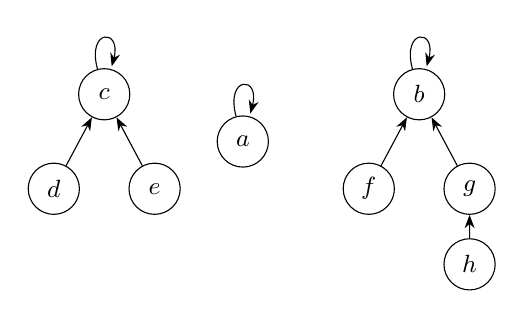
\begin{tikzpicture}[scale=.8,
      vertice/.style={circle, draw, minimum size=6.5mm, inner sep=0pt, font=\small},
      every edge/.style={draw, ->}]
    \node[vertice] (c) at (0, 1.5) {$c$};
    \path (c) edge [loop above] (c);
    \node[vertice] (d) at (-0.8, 0) {$d$};
    \node[vertice] (e) at (0.8, 0) {$e$};
    \draw[->] (d) -- (c);  \draw[->] (e) -- (c);
    \node[vertice] (a) at (2.2, 0.75) {$a$};
    \path (a) edge [loop above] (a);
    \node[vertice] (b) at (5.0, 1.5) {$b$};
    \path (b) edge [loop above] (b);
    \node[vertice] (f) at (4.2, 0) {$f$};
    \node[vertice] (g) at (5.8, 0) {$g$};
    \node[vertice] (h) at (5.8, -1.2) {$h$};
    \draw[->] (f) -- (b);  \draw[->] (g) -- (b);  \draw[->] (h) -- (g);
  \end{tikzpicture}

  {\footnotesize Representação com árvores de $\{c,d,e\}$, $\{a\}$ e
    $\{b,f,g,h\}$.}
\end{frame}

% =====================================================================
\begin{frame}[t]{Floresta: o problema e a união por tamanho}
\vfill
  \begin{minipage}[c]{.5\linewidth}
    \centering
    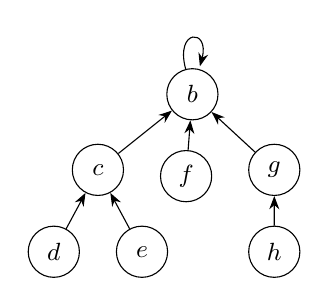
\begin{tikzpicture}[scale=.8,
        vertice/.style={circle, draw, minimum size=6.5mm, inner sep=0pt, font=\small},
        every edge/.style={draw, ->}]
      \node[vertice] (b) at (0, 2) {$b$};
      \path (b) edge [loop above] (b);
      \node[vertice] (c) at (-1.5, 0.8) {$c$};
      \node[vertice] (f) at (-0.1, 0.7) {$f$};
      \node[vertice] (g) at (1.3, 0.8) {$g$};
      \node[vertice] (d) at (-2.2, -0.5) {$d$};
      \node[vertice] (e) at (-0.8, -0.5) {$e$};
      \node[vertice] (h) at (1.3, -0.5) {$h$};
      \draw[->] (d) -- (c);  \draw[->] (e) -- (c);  \draw[->] (c) -- (b);
      \draw[->] (f) -- (b);  \draw[->] (h) -- (g);  \draw[->] (g) -- (b);
    \end{tikzpicture}

    {\footnotesize Resultado de $\Uniao(e,f)$: a raiz $c$ (tamanho $3$)
      é pendurada na raiz $b$ (tamanho $4$).}
  \end{minipage}
  \hfill
  \begin{minipage}[c]{.47\linewidth}
    Essa estrutura pode ser muito ruim: se pendurarmos sempre a raiz da
    árvore maior numa árvore unitária, formamos uma cadeia com $n$ nós,
    em que cada busca no nó mais profundo custa $\Theta(n)$.
  \end{minipage}

 \end{frame}

% =====================================================================
\begin{frame}[c]{Floresta: o problema e a união por tamanho}

  O \alert{\textit{tamanho}} de uma árvore é o seu número de nós.
  
  \vfill
  
  A \alert{\textit{altura}} de uma árvore é a maior distância de um nó
  até a raiz.
  
  \vfill
  
  \begin{block}{União por tamanho}
    A raiz da árvore de menor tamanho é pendurada na raiz da árvore de
    maior tamanho (em caso de empate, em qualquer uma).
  \end{block}

  \vfill
  
    Qual a relação entre tamanho e altura após uma sequência de uniões
    com essa heurística?  \vfill
  

\end{frame}

% =====================================================================
\begin{frame}[t]{Floresta: algoritmos com união por tamanho}

  Cada nó tem $\mathrm{pai}[x]$ e, nas raízes, $t[x]$ = número de
  elementos da árvore enraizada em $x$.

  \medskip
  \begin{minipage}[t]{.3\linewidth}
    \textbf{cria$(x)$}
    \begin{algorithmic}[1]
      \State $\mathrm{pai}[x]\gets x$
      \State $t[x]\gets1$
    \end{algorithmic}
  \end{minipage}
  \hfill
  \begin{minipage}[t]{.33\linewidth}
    \textbf{busca$(x)$}
    \begin{algorithmic}[1]
      \While{$x\neq\mathrm{pai}[x]$}
      \State $x\gets\mathrm{pai}[x]$
      \EndWhile
      \State \Return $x$
    \end{algorithmic}
  \end{minipage}
  \hfill
  \begin{minipage}[t]{.3\linewidth}
    \textbf{link$(x,y)$}
    \begin{algorithmic}[1]
      \State $t[x]\gets t[x]+t[y]$
      \State $\mathrm{pai}[y]\gets x$
    \end{algorithmic}
  \end{minipage}

  \medskip
  $\Link$ pressupõe que $x$ e $y$ são raízes distintas com
  $t[x]\geq t[y]$ (garantido por $\Uniao$); $\Uniao$ pressupõe que $x$ e
  $y$ estão em árvores distintas.

  \medskip
  \textbf{uniao$(x,y)$}
  \begin{algorithmic}[1]
    \State $r_x\gets\Busca(x)$;\ \ $r_y\gets\Busca(y)$
    \If{$t[r_x]\geq t[r_y]$} \State $\Link(r_x,r_y)$
    \Else\ \State $\Link(r_y,r_x)$
    \EndIf
  \end{algorithmic}
\end{frame}

% =====================================================================
\begin{frame}[t]{União por tamanho: tamanho $\times$ altura}

  \begin{block}{Proposição}
    Usando união por tamanho, e supondo que as $n$ primeiras operações
    são $\Cria$, em qualquer momento cada árvore tem pelo menos $2^h$
    nós, onde $h$ é a sua altura.
  \end{block}\pause
  \begin{proof}[Prova]
    \small
    Indução no número $k$ de uniões já realizadas.  Para $k=0$, as
    únicas operações até então que alteram a estrutura são $\Cria$, e
    toda árvore tem um nó e altura $0$, com $1\geq2^0$.  Seja $k\geq1$:
    como as $n$ primeiras operações são $\Cria$, nada além das uniões
    altera a estrutura.  A $k$-ésima união liga duas árvores distintas
    $A$ e $B$, com tamanhos $t_A,t_B$ e alturas $h_A,h_B$; por indução
    $t_A\geq2^{h_A}$ e $t_B\geq2^{h_B}$.  Sem perda de generalidade
    $t_A\geq t_B$ e a raiz de $B$ é pendurada na de $A$.  A árvore
    resultante tem $t'=t_A+t_B$ nós e altura $h'=\max\{h_A,h_B+1\}$.
    \begin{itemize}
    \item Se $h'=h_A$: $t'\geq t_A\geq2^{h_A}=2^{h'}$.
    \item Se $h'=h_B+1$: $t'=t_A+t_B\geq2t_B\geq2\cdot2^{h_B}=2^{h'}$.
    \end{itemize}
  \end{proof}
\end{frame}

\begin{frame}[t]{União por tamanho: custo}
  \begin{block}{Corolário}
    Usando união por tamanho, com as $n$ primeiras operações $\Cria$, o
    tempo de $m$ operações é $O(m(1+\log n))$.
  \end{block}
  \begin{proof}[Prova]
    Pela proposição, uma árvore de altura $h$ tem $2^h\leq n$ nós, logo
    $h\leq\log_2n$ e cada $\Busca$ custa $O(1+\log n)$.  Cada $\Cria$
    custa $O(1)$ e cada $\Uniao$ custa duas buscas mais $O(1)$, isto é,
    $O(1+\log n)$.  O total é $O(n+m(1+\log n))=O(m(1+\log n))$, pois
    $m\geq n$.
  \end{proof}
  \begin{alertblock}{Kruskal com floresta}
    Com $m=O(|E|)$ e $n=|V|$, o custo das operações é
    $O(|E|\log|V|)$; somado à ordenação, o tempo total é
    $O(|E|\log|V|)$.
  \end{alertblock}
\end{frame}

% =====================================================================
\begin{frame}[c]{União por altura e por \textit{rank}}

  Como o tempo de $\Busca$ é proporcional à altura da árvore, parece
  mais natural uma heurística baseada na altura. \pause
  \begin{block}{União por altura}
    A raiz da árvore mais baixa é pendurada na raiz da árvore mais alta
    (em caso de empate, em qualquer uma).
  \end{block}
  Cada raiz $r$ guarda $h[r]$, a altura da árvore enraizada em $r$,
  iniciada com $0$.  $\Link$ pressupõe raízes distintas com
  $h[x]\geq h[y]$.

  \medskip
  \begin{minipage}[t]{.3\linewidth}
    \textbf{cria$(x)$}
    \begin{algorithmic}[1]
      \State $\mathrm{pai}[x]\gets x$
      \State $h[x]\gets0$
    \end{algorithmic}
  \end{minipage}
  \hfill
  \begin{minipage}[t]{.37\linewidth}
    \textbf{link$(x,y)$ (por altura)}
    \begin{algorithmic}[1]
      \If{$h[x]=h[y]$} \State $h[x]\gets h[x]+1$ \EndIf
      \State $\mathrm{pai}[y]\gets x$
    \end{algorithmic}
  \end{minipage}
  \hfill
  \begin{minipage}[t]{.3\linewidth}
    \textbf{uniao$(x,y)$}
    \begin{algorithmic}[1]
      \State $r_x\gets\Busca(x)$;\State  $r_y\gets\Busca(y)$
      \If{$h[r_x]\geq h[r_y]$} \State $\Link(r_x,r_y)$
      \Else\ \State $\Link(r_y,r_x)$ \EndIf
    \end{algorithmic}
  \end{minipage}
 \hfill \hfill
 \hfill \hfill
 \end{frame}

% =====================================================================
\begin{frame}[c]{Floresta: por que a altura fica pequena?}

  \textbf{Ideia:} a altura só aumenta quando pendurada
  uma árvore de \textit{mesma altura}.  Portanto, uma árvore de altura
  $h$ foi montada a partir de \textbf{duas de altura $h-1$}:

  \medskip
  \centering
  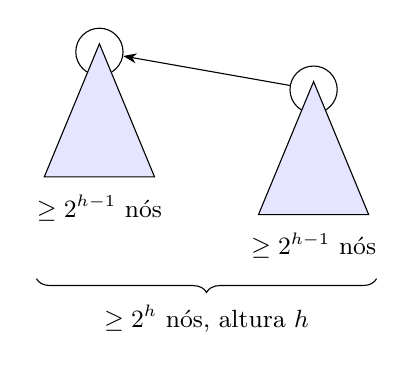
\begin{tikzpicture}[scale=.8,
      vertice/.style={circle,draw,minimum size=6mm,inner sep=0pt,font=\small},
      subtree/.style={isosceles triangle,draw,shape border rotate=90,
        minimum width=14mm,minimum height=11mm,inner sep=0pt,fill=blue!10}]
    \node[vertice] (r) at (0,2.4) {};
    \node[vertice] (s) at (3.4,1.8) {};
    \node[subtree] (A) at (0,1.0) {};
    \node[subtree] (B) at (3.4,0.4) {};
    \draw[->] (s) -- (r);
    \node[font=\small,below=1mm of A] {$\geq2^{h-1}$ nós};
    \node[font=\small,below=1mm of B] {$\geq2^{h-1}$ nós};
    \draw[decorate,decoration={brace,mirror,amplitude=5pt}] (-1,-1.2) -- (4.4,-1.2)
      node[midway,below=6pt,font=\small] {$\geq2^{h}$ nós, altura $h$};
  \end{tikzpicture}

  \smallskip
  \raggedright
  Logo uma árvore de altura $h$ tem $\geq2^h$ nós; com no máximo $n$
  nós, a altura é $\leq\log_2n$.  Cada $\Busca$ custa $O(\log n)$ e

\end{frame}

% =====================================================================
\begin{frame}[c]{União por altura e por \textit{rank}}
 \vfill
  Valem os mesmos resultados:

   \vfill

  \begin{block}{Proposição}
    Usando união por altura, e supondo que as $n$ primeiras operações
    são $\Cria$, em qualquer momento cada árvore tamanho$\geq 2^h$ nós,
    onde $h$ é a sua altura.
  \end{block}

  \vfill
  
  \begin{block}{Corolário}
    Usando união por altura, com as $n$ primeiras operações $\Cria$, o
    tempo de $m$ operações é $O(m(1+\log n))$.
  \end{block}

   \vfill
\end{frame}

% =====================================================================
\begin{frame}[c]{Busca com compressão de caminhos e união por \textit{rank}}

  \medskip
  
  Quando introduzirmos compressão de caminhos, $h$ deixa de ser a
  altura exata: passa a se chamar \textbf{rank}.

  \pause
  
  \begin{block}{Compressão de caminhos}
    Quando fazemos $\Busca(x)$, aproveitamos o percurso de $x$ até a
    raiz e desviamos os ponteiros $\mathtt{pai}[y]$, de todo $y$ nesse
    caminho, para a raiz; na união penduramos a árvore de menor
    \textit{rank} na raiz da de maior \textit{rank}.
  \end{block}

  \centering
  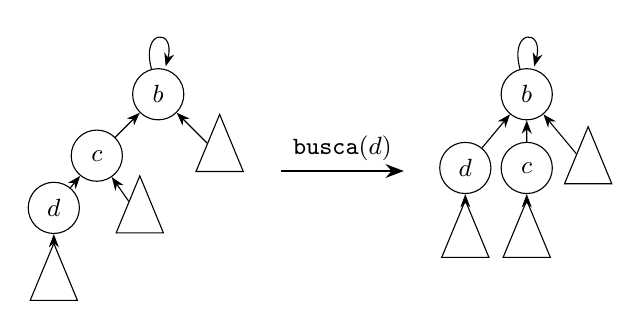
\begin{tikzpicture}[scale=.78,
      vertice/.style={circle, draw, minimum size=6.5mm, inner sep=0pt, font=\small},
      subtree/.style={isosceles triangle, draw, shape border rotate=90,
        minimum width=6mm, minimum height=7mm, inner sep=0pt},
      every edge/.style={draw, ->}]
    % antes
    \node[vertice] (b1) at (0, 2.5) {$b$};
    \path (b1) edge [loop above] (b1);
    \node[vertice] (c1) at (-1, 1.5) {$c$};
    \node[vertice] (d1) at (-1.7, 0.65) {$d$};
    \node[subtree] (s11) at (-1.7, -0.6) {};
    \node[subtree] (s12) at (-0.3, 0.5) {};
    \node[subtree] (s13) at (1, 1.5) {};
    \draw[->] (s11) -- (d1);
    \draw[->] (d1) -- (c1);
    \draw[->] (s12) -- (c1);
    \draw[->] (c1) -- (b1);
    \draw[->] (s13) -- (b1);
    % seta
    \draw[->, thick] (2, 1.25) -- (4, 1.25)
      node[midway, above, font=\small] {$\Busca(d)$};
    % depois
    \node[vertice] (b2) at (6, 2.5) {$b$};
    \path (b2) edge [loop above] (b2);
    \node[vertice] (c2) at (6, 1.3) {$c$};
    \node[vertice] (d2) at (5, 1.3) {$d$};
    \node[subtree] (s21) at (5, 0.1) {};
    \node[subtree] (s22) at (6, 0.1) {};
    \node[subtree] (s23) at (7, 1.3) {};
    \draw[->] (s21) -- (d2);  \draw[->] (d2) -- (b2);
    \draw[->] (s22) -- (c2);  \draw[->] (c2) -- (b2);
    \draw[->] (s23) -- (b2);
  \end{tikzpicture}

  {\footnotesize Esquema de uma busca com compressão de caminhos: $d$ e
    $c$ passam a ser filhos da raiz $b$.}
\end{frame}

% =====================================================================
\begin{frame}[c]{\textit{Rank} e os algoritmos}

    \vfill
  
  A compressão encurta caminhos, e manter a altura exata a cada busca
  seria caro.  Em vez disso guardamos em cada raiz um \textbf{rank}:
  \begin{itemize}
  \item começa em $0$ e só muda numa união: se as duas raízes têm o
    mesmo rank, a que recebe sobe $1$;
  \item é uma \textbf{cota superior} da altura (igual a ela quando não
    há compressão);
  \item um nó de rank $r$ tem pelo menos $2^r$ descendentes, como no
    argumento da altura: então $\mathrm{rank}\leq\log_2n$.
  \end{itemize}


  \vfill
  
  \begin{block}{Duas propriedades que usaremos}
    \begin{enumerate}[(a)]
    \item Todo ancestral próprio de $x$ tem rank \textbf{estritamente
        maior} que o de $x$.
    \item Depois que deixa de ser raiz, o rank de um nó \textbf{nunca
        mais muda}; o rank do \textit{pai} de $x$ só pode aumentar
      (ou ficar igual) ao longo do tempo.
    \end{enumerate}
  \end{block}
  
    \vfill
 \end{frame}

% =====================================================================
\begin{frame}[t]{\textit{Rank} e os algoritmos}
  
  \begin{minipage}[t]{.43\linewidth}
    \textbf{cria$(x)$}
    \begin{algorithmic}[1]
      \State $\mathrm{pai}[x]\gets x$
      \State $\mathrm{rank}[x]\gets0$
    \end{algorithmic}
  \end{minipage}
  \hfill
  \begin{minipage}[t]{.53\linewidth}
    \textbf{busca$(x)$ com compressão}
    \begin{algorithmic}[1]
      \If{$x\neq\mathrm{pai}[x]$}
      \State $\mathrm{pai}[x]\gets\Busca(\mathrm{pai}[x])$
      \EndIf
      \State \Return $\mathrm{pai}[x]$
    \end{algorithmic}
  \end{minipage}

  \bigskip
  \begin{minipage}[t]{.43\linewidth}
    \textbf{link$(x,y)$}
    \begin{algorithmic}[1]
      \If{$\mathrm{rank}[x]=\mathrm{rank}[y]$}
      \State $\mathrm{rank}[x]\gets\mathrm{rank}[x]+1$
      \EndIf
      \State $\mathrm{pai}[y]\gets x$
    \end{algorithmic}
  \end{minipage}
  \hfill
  \begin{minipage}[t]{.53\linewidth}
    \textbf{uniao$(x,y)$}
    \begin{algorithmic}[1]
      \State $r_x\gets\Busca(x)$;\ \ $r_y\gets\Busca(y)$
      \If{$\mathrm{rank}[r_x]\geq\mathrm{rank}[r_y]$}
      \State $\Link(r_x,r_y)$
      \Else
      \State $\Link(r_y,r_x)$
      \EndIf
    \end{algorithmic}
  \end{minipage}

  \bigskip
  $\Link$ pressupõe que $x$ e $y$ são raízes distintas com
  $\mathrm{rank}[x]\geq\mathrm{rank}[y]$ (garantido por $\Uniao$), e
  $\Uniao$ que $x$ e $y$ estão em árvores distintas.
\end{frame}

% =====================================================================
\begin{frame}[t]{O resultado de Tarjan e a função $\alpha$}
  \small
  \begin{block}{Teorema (Tarjan, 1975)}
    Com união por rank e compressão de caminhos, o tempo gasto com $m$
    operações num universo de tamanho $n$, com $m\geq n$ (as $n$
    primeiras sendo $\Cria$), é $O(m\,\alpha(m,n))$.
  \end{block}
  Não demonstraremos esse teorema (veja CLR); o resultado que
  mostraremos é um pouco menos preciso.

  \medskip
  A função de Ackermann (versão de CLR), para $i,j\geq1$:
  \[
    A(i,j)=
    \begin{cases}
      2^j & \text{se } i=1,\\
      A(i-1,2) & \text{se } i\geq2 \text{ e } j=1,\\
      A\big(i-1,A(i,j-1)\big) & \text{se } i\geq2 \text{ e } j\geq2,
    \end{cases}
    \qquad
    \alpha(m,n)=\min\big\{i\geq1\colon A(i,\lfloor m/n\rfloor)>\log_2n\big\}.
  \]
  \footnotesize
  $A(2,j)$ é uma torre de exponenciais com $j+1$ dois, $A(3,1)=16$ e
  $A(4,1)=A(2,16)$ é uma torre de $17$ dois, imensamente maior que
  $10^{80}$.  Como $A$ é crescente em $j$, $\alpha(m,n)\leq\alpha(n,n)$,
  e portanto $\alpha(m,n)\leq4$ para todo $n<2^{A(4,1)}$.

  \centering
  \begin{tabular}{|r|c|}\hline
    $n$ & $\alpha(n,n)$ \\ \hline\hline
    $1$ -- $3$ & $1$ \\ \hline
    $4$ -- $15$ & $2$ \\ \hline
    $16$ -- $65535$ & $3$ \\ \hline
    $65536$ -- $2^{A(4,1)}-1$ & $4$ \\ \hline
  \end{tabular}
\end{frame}

% =====================================================================
\begin{frame}[c]{Análise (1/3): poucos nós têm rank alto}
  Um nó de rank $r$ ``traz junto''\footnote{árvore \textbf{no momento em que ele deixa de ser raiz} (depois disso a
compressão pode encolher a subárvore, mas esse conjunto fica fixo).} pelo menos $2^r$ elementos, e
  esses elementos \textbf{não são reaproveitados} por outro nó do mesmo
  rank.  Logo, há no máximo $n/2^r$ nós de rank $r$:

  \medskip
  \centering
  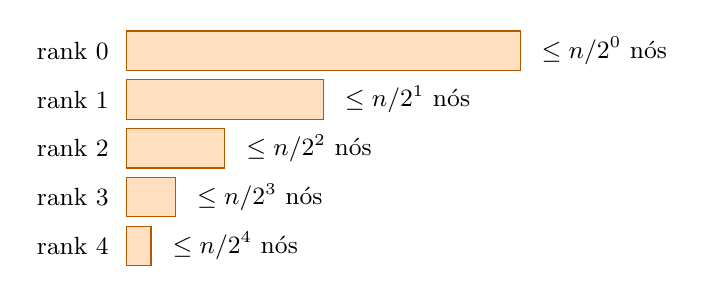
\begin{tikzpicture}
    \foreach \r in {0,1,2,3,4} {
      \pgfmathsetmacro{\w}{5/(2^\r)}
      \draw[fill=orange!25,draw=orange!70!black] (0,-0.62*\r) rectangle (\w,-0.62*\r+0.5);
      \node[anchor=east,font=\small] at (-0.1,-0.62*\r+0.25) {rank $\r$};
      \node[anchor=west,font=\small] at (\w+0.15,-0.62*\r+0.25) {$\leq n/2^{\r}$ nós};
    }
  \end{tikzpicture}

  \medskip
  \raggedright
  É uma \textbf{pirâmide}: metade dos nós tem rank baixo, e os ranks altos
  são raros.  Em particular, os nós de rank maior que $j$ são no máximo
  $n/2^j$.
\end{frame}
% =====================================================================
\begin{frame}[c]{Análise (2/3): agrupar os ranks em faixas}

  Considere $m$ operações, as $n$ primeiras $\Cria$, com união por
  \textit{rank} e compressão.  Sejam
  \begin{center}
    $b_0=1$ e $b_g=2^{b_{g-1}}$
  \end{center}
  isto é, $1,2,4,16,65536,\dots$

  \bigskip
  
  Particionamos $\mathcal U$ em \textbf{grupos} segundo o \textit{rank
    final}:
  \begin{itemize}
  \item Grupo $0$: elementos de rank $0$ e $1$;
  \item Grupo $1$: elementos de rank em $(1,2]$;
  \item Grupo $2$: elementos de rank em $(2,4]$;
  \item Grupo $3$: elementos de rank em $(4, 16]$;
  \item Grupo $4$: elementos de rank em $(16, 65536]$;
  \item $\vdots$
  \item Grupo $g\geq1$: elementos de rank em $(b_{g-1},b_g]=(K,2^K]$.
  \end{itemize}
 \end{frame}
% =====================================================================
\begin{frame}[c]{Análise (2/3): agrupar os ranks em faixas}

  Dividimos os ranks possíveis ($0,\dots,\log_2n$) em \textbf{faixas}
  que ficam cada vez mais largas: a faixa $g$ cobre os ranks
  $(K,2^K]$, com $K$ o fim da faixa anterior.

  \medskip
  \centering
  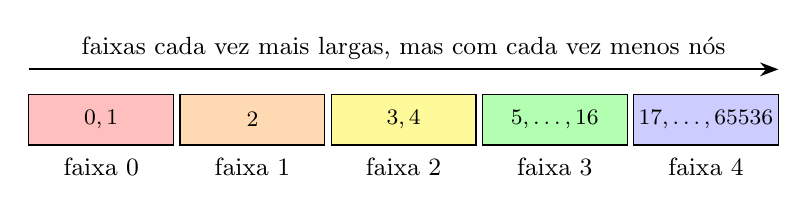
\begin{tikzpicture}[scale=.8]
    \foreach \x/\lab/\c/\g in {0/{$0,1$}/red!25/0, 2.4/{$2$}/orange!30/1,
        4.8/{$3,4$}/yellow!40/2, 7.2/{$5,\dots,16$}/green!30/3,
        9.6/{$17,\dots,65536$}/blue!20/4} {
      \draw[fill=\c] (\x,0) rectangle (\x+2.3,0.8);
      \node[font=\footnotesize] at (\x+1.15,0.4) {\lab};
      \node[font=\small] at (\x+1.15,-0.35) {faixa \g};
    }
    \draw[->,thick] (0,1.2) -- (11.9,1.2) node[midway,above,font=\small]
      {faixas cada vez mais largas, mas com cada vez menos nós};
  \end{tikzpicture}

  \medskip
  \raggedright
  A largura \textbf{explode} (de $K$ para $2^K$), então bastam
  $\lgs n$ faixas para cobrir todos os ranks.

  \bigskip

  \textbf{Compromisso:} faixa mais larga $\Rightarrow$ um nó dela pode
  ser contado em mais buscas (o pai dele passa por mais ranks sem
  sair da faixa), mas a pirâmide garante que há menos nós
  nela. 
\end{frame}
% =====================================================================
\begin{frame}[t]{Análise (3/3): que nós são contados em cada busca?}
  \small
  O custo de uma busca é o número de nós do caminho percorrido: \textbf{contamos
    $O(1)$ para cada nó}.  Separamos os nós do caminho em dois tipos e
  limitamos quantas vezes cada tipo pode ser contado:
 
  \medskip
  \begin{block}{Tipo 1: a raiz, o filho da raiz, ou quem \textbf{troca de faixa} para o pai}
    No caminho o rank só cresce, então o caminho cruza no máximo
    $\lgs n$ faixas: \textbf{$\leq\lgs n+1$ nós por busca}, em
    $O(m\lgs n)$ ao todo.
  \end{block}
 
  \begin{block}{Tipo 2: $y$ e o pai estão na \textbf{mesma} faixa}
    Cada vez que $y$ é contado como Tipo 2, ele passa a apontar para a
    raiz, que tem rank \textbf{maior} que o do pai anterior.  Como a
    faixa tem no máximo $2^K$ ranks, $y$ é contado no máximo $2^K$ vezes
    e depois seu pai sai da faixa.  A faixa tem no máximo $n/2^K$ nós:
    \[
      \underbrace{\frac{n}{2^K}}_{\text{nós}}\cdot
      \underbrace{2^K}_{\text{vezes contado por nó}}=n
      \qquad\Rightarrow\qquad \text{cada faixa custa }n.
    \]
    Com $\lgs n$ faixas: $O(n\lgs n)$.
  \end{block}

\end{frame}

% % % =====================================================================
% % \begin{frame}[c]{Um resultado mais fraco: grupos de \textit{rank}}
% % 
% %   Considere $m$ operações, as $n$ primeiras $\Cria$, com união por
% %   \textit{rank} e compressão.  Sejam
% %   \begin{center}
% %     $b_0=1$ e $b_g=2^{b_{g-1}}$
% %   \end{center}
% %   isto é, $1,2,4,16,65536,\dots$
% % 
% %   \bigskip
% %   
% %   Particionamos $\mathcal U$ em \textbf{grupos} segundo o \textit{rank
% %     final}:
% %   \begin{itemize}
% %   \item Grupo $0$: elementos de rank $0$ e $1$;
% %   \item Grupo $1$: elementos de rank em $(1,2]$;
% %   \item Grupo $2$: elementos de rank em $(2,4]$;
% %   \item Grupo $3$: elementos de rank em $(4, 16]$;
% %   \item Grupo $4$: elementos de rank em $(16, 65536]$;
% %   \item $\vdots$
% %   \item Grupo $g\geq1$: elementos de rank em $(b_{g-1},b_g]=(K,2^K]$.
% %   \end{itemize}
% %  \end{frame}
% % 
% % % =====================================================================
% %  \begin{frame}[c]{Um resultado mais fraco: grupos de \textit{rank}}
% %    
% %  \begin{block}{Propriedades do \textit{rank}}
% %     \begin{enumerate}[(i)]\itemsep=.5cm
% %     \item o rank de um nó só muda em $\Link$, quando ele é a raiz que
% %       recebe a outra; depois que deixa de ser raiz, não muda mais;
% %     \item $\mathrm{rank}[x]<\mathrm{rank}[\mathrm{pai}[x]]$ para todo
% %       $x$ que não é raiz; em particular,
% %       $\mathrm{rank}[\mathrm{pai}[x]]$ não decresce ao longo do tempo;
% %     \item se $x\neq y$ têm o mesmo rank final, então
% %       $D(x)\cap D(y)=\emptyset$, e $|D(x)|\geq2^{\mathrm{rank}[x]}$,
% %       onde $D(x)$ é a árvore de $x$ no instante em que $x$ deixa de ser
% %       raiz (ou no fim);
% %     \item para todo $k$, há no máximo $n/2^k$ nós de rank maior que $k$;
% %       em particular, o Grupo $g$ tem no máximo $n/2^K$ nós;
% %     \item há no máximo $\lgs n$ grupos.
% %     \end{enumerate}
% %   \end{block}
% % \end{frame}
% % 
% % % =====================================================================
% % \begin{frame}[c]{Justificativa de (ii) e (iii)}
% % 
% % 
% %   \bigskip
% %   
% %   \textbf{(ii)} Vale na criação; em $\Link$, se os ranks são iguais o
% %   da raiz que recebe aumenta; e a compressão aponta $x$ para um
% %   ancestral, de rank maior.  Logo $\mathrm{rank}[\mathrm{pai}[x]]$ só
% %   aumenta.
% % 
% %   \bigskip
% %   
% %   \textbf{(iii)} A árvore de $x$ no instante em que deixa de ser raiz
% %   tem pelo menos $2^{\mathrm{rank}[x]}$ nós (proposição com rank), e o
% %   seu rank já é o final por (i).
% % 
% %   Suponha $z\in D(x)\cap D(y)$, com $x\neq y$ do mesmo rank $r$ e, sem
% %   perda de generalidade, $x$ deixando de ser raiz antes de $y$ (ou $y$
% %   sendo raiz no fim).
% %   
% %   \begin{itemize}\itemsep=.3cm
% %   \item Nesse instante $x$ é ligado a uma raiz $R$ de rank $\geq r$;
% %     após o $\Link$ a raiz da árvore de $z$ passa a ter rank $>r$ (se
% %     $\mathrm{rank}[R]=r$, ele aumenta), e esse rank só cresce.
% %   \item Quando $y$ deixa de ser raiz, $y$ é a raiz da árvore de $z$ com
% %     rank $r$: contradição.
% %   \end{itemize}
% % \end{frame}
% % 
% % % =====================================================================
% % \begin{frame}[c]{Justificativa de (iv) e (v)}
% % 
% %   \bigskip
% % 
% %   
% %   \textbf{(iv)} Para cada $r$, os $D(x)$ de rank $r$ são disjuntos e têm
% %   $\geq2^r$ elementos, logo há $\leq n/2^r$ nós de rank $r$.  Somando
% %   sobre $r>k$:
% %   \[
% %     \sum_{r>k}\frac{n}{2^r}=\frac{n}{2^k}.
% %   \]
% % 
% %     \bigskip
% % 
% % 
% %   \textbf{(v)} O rank é no máximo $\lfloor\lg n\rfloor$ (proposição).
% %   Se $g_0$ é o menor $g$ com $b_g\geq\lfloor\lg n\rfloor$, há $g_0+1$
% %   grupos.  Para $g_0\geq1$ vale $b_{g_0-1}<\lg n$, isto é,
% %   $n>2^{b_{g_0-1}}=b_{g_0}$.  Aplicando $\lg$ repetidamente,
% %   \[
% %     \lg^{(g_0)}n>\lg^{(g_0)}b_{g_0}=b_0=1,
% %   \]
% %   logo $\lgs n\geq g_0+1$.
% % \end{frame}
% % 
% % % =====================================================================
% % \begin{frame}[c]{Custo das buscas: nós de dois tipos}
% % 
% % 
% %   
% %   O custo total é $O(m)$ ($\Cria$ e $\Link$ custam $O(1)$) mais o custo
% %   das $f\leq2m$ buscas.  O custo de uma busca é o número de nós do
% %   caminho $x=y_0,\dots,y_k$ até a raiz, cujos apontadores são
% %   redirecionados.  Classificamos os nós $y$ do caminho:
% %   \begin{enumerate}
% %   \item \textbf{Tipo 1:} $y$ é a raiz ou filho da raiz, ou
% %     $\mathrm{pai}[y]$ está em grupo diferente do de $y$;
% %   \item \textbf{Tipo 2:} os demais, isto é, $y$ não é a raiz nem filho
% %     da raiz e $\mathrm{pai}[y]$ está no mesmo grupo que $y$.
% %   \end{enumerate}
% % 
% %   \bigskip
% %   
% %   \begin{block}{Tipo 1}
% %     Ao longo do caminho o rank cresce estritamente, logo o grupo não
% %     decresce e muda no máximo $\lgs n-1$ vezes; com a raiz e o filho da
% %     raiz, cada busca tem no máximo $\lgs n+1$ nós do Tipo 1.  Em $f$
% %     buscas são
% %     \[
% %       O(m\lgs n).
% %     \]
% %   \end{block}
% % \end{frame}
% % 
% % % =====================================================================
% % \begin{frame}[c]{Nós do Tipo 2}
% % 
% %   Seja $y$ no Grupo $g\geq1$, com ranks em $(K,2^K]$.  Cada vez que $y$
% %   é do Tipo 2 em uma busca, $\mathrm{pai}[y]$ passa a ser a raiz, cujo
% %   rank é maior que o do pai anterior (pois este não era a raiz).  Como o
% %   rank do pai só cresce e o de $y$ é fixo por (i):
% % 
% %   \bigskip
% % 
% %   \begin{itemize}
% %   \item o rank de $\mathrm{pai}[y]$ assume valores distintos em
% %     $(\mathrm{rank}[y],2^K]$ a cada ocorrência;
% %   \item depois que sai do grupo, $y$ nunca mais é do Tipo 2.
% %   \end{itemize}
% % 
% %     \bigskip
% % 
% %   Logo $y$ é do Tipo 2 no máximo $2^K$ vezes.  Por (iv) há no máximo
% %   $n/2^K$ tais nós, e o Grupo $g$ contribui com no máximo
% %   \[
% %     \frac{n}{2^K}\cdot2^K=n.
% %   \]
% % 
% %     \bigskip
% % 
% %   
% %   No Grupo $0$ cada nó é do Tipo 2 no máximo uma vez (o pai precisa ter
% %   rank $1$, e depois o pai passa para fora do grupo): contribui com no
% %   máximo $n$.  Somando sobre os $\leq\lgs n$ grupos,
% %   \[
% %     O(n\lgs n).
% %   \]
% % \end{frame}
% % 
% % % =====================================================================
% % \begin{frame}[c]{O teorema}
% % 
% %   
% %   \begin{block}{Teorema}
% %     Com união por \textit{rank} e compressão de caminhos, o tempo gasto
% %     com $m$ operações $\Cria$/$\Busca$/$\Uniao$ num universo com $n$
% %     elementos, das quais as $n$ primeiras são $\Cria$, é
% %     \[
% %       O\big((m+n)\lgs n\big).
% %     \]
% %   \end{block}
% % 
% %     \bigskip
% % 
% % 
% %   \textbf{Resumo da prova:} $O(m)$ para $\Cria$ e $\Link$, mais
% %   $O(m\lgs n)$ para os nós do Tipo 1, mais $O(n\lgs n)$ para os do
% %   Tipo 2.
% % 
% %   \bigskip
% % 
% %   \textbf{No Kruskal:} com $m=O(|E|)$ operações e $n=|V|\leq|E|+1$, o
% %   custo das operações é $O(|E|\lgs|V|)$, dominado pela ordenação das
% %   arestas:
% %   \[
% %     O(|E|\log|E|)=O(|E|\log|V|).
% %   \]
% % \end{frame}
% % 
% =====================================================================
\begin{frame}[c]{Resumo: $m$ operações ($n$ primeiras $\Cria$) e Kruskal}

  \centering
  \renewcommand{\arraystretch}{1.4}
  \begin{tabular}{|l|c|c|}\hline
    \textbf{Estrutura} & \textbf{Tempo de $m$ operações} &
                                                           \textbf{Kruskal} \\ \hline\hline
    Vetor & $O(m+n^2)$ & $O(|E|\log|E|+|V|^2)$ \\ \hline
    Listas ligadas + menor lista & $O(m+n\log n)$ & $O(|E|\log|V|)$ \\ \hline
    Floresta, união por tamanho/altura & $O(m(1+\log n))$ &
                                                            $O(|E|\log|V|)$ \\ \hline
    Floresta, rank + compressão & $O((m+n)\lgs n)$
                                  {\scriptsize\ (Tarjan: $O(m\,\alpha(m,n))$)} & $O(|E|\log|V|)$ \\ \hline
  \end{tabular}

  \medskip\normalsize
  Com listas ou florestas, a ordenação das arestas passa a dominar o
  custo do Kruskal; a estrutura de dados deixa de ser o gargalo.
\end{frame}

\end{document}

%%% Local Variables:
%%% mode: LaTeX
%%% TeX-master: t
%%% End:
